\documentclass[11pt, final]{article}

\usepackage{amssymb} \usepackage{amsmath} \usepackage{amsthm} \usepackage{algorithm} \usepackage{algorithmic} \usepackage{url} \usepackage[margin=1in]{geometry} \usepackage{graphicx} \usepackage{subfigure} \usepackage{color}
\usepackage{hyperref}


\usepackage{graphicx}
\usepackage{epstopdf}

\newtheorem{theorem}{Theorem} \newtheorem{lemma}{Lemma} \newtheorem{corollary}{Corollary} \newtheorem{definition}{Definition} \newtheorem{assumption}{Assumption} \newtheorem{example}{Example}
\newtheorem{observation}[theorem]{Observation}
\usepackage{enumerate}

\usepackage{color}
\newcounter{todocounter}
\newcommand{\todo}[1]{\stepcounter{todocounter}\textcolor{red}{to-do\#\arabic{todocounter}: #1}}

\graphicspath{{../figs/}}

\begin{document}

\title{CS659: HW1}



\date{02/15/2015}

\maketitle

%%%%%%%%%%%%%%%%%%%%%%%%%%%%%%%%%%%%%%%%%%%%%%%%%%%%%%%%%%%%%%%%%%%%%%%%%%%%%%%%
\paragraph{\text{1. }} Given the data set found in the file \href{http://cs.gmu.edu/~dbarbara/CS659/z.txt}{z}

\begin{enumerate}[(a)]
\item Use the first 99 records to compute the covariance matrix $\sum$ \\

\textbf{Answer:} Denote the first column and second column as $X$ and $Y$, then $Cov(X,Y) = \sum (X_i - \bar{X}) (Y_i - \bar{Y}) /N$, 

\begin{displaymath}
Cov(X,Y) = 
\begin{bmatrix}
    1.729 &  0.837 \\
    0.837 &  1.599 \\
\end{bmatrix}
\end{displaymath}



 
\item The centroid of those 99 records, which is computed as a record whose attributes values are the average of the other record values\\

\textbf{Answer:} The centroid is ($3.965$
$4.960$).
\item Using the result of a), compute
\begin{enumerate}[(i)]
\item The mahalanobis distance of records 100, 101 and 102 to the centroid computed in b)\\

\textbf{Answer:} The mahalanobis distance between two nodes x and y is $D = \sqrt{(x-y)^T S^{-1} (x-y)}$ where $S$ is the co-variance metrix. \\
Thus the mahalanobis distance for records 100, 101, and 102 are: $3.409$, $ 4.982$, $5.449$. 

\item Repeat i) but compute the Euclidean distance \\

\textbf{Answer:} The Euclidean distance between two nodes x and y is $D = \sqrt{\sum^n_{i=1} (x_i - y_i)^2}$. \\
Thus the Euclidean distance for records 100, 101, and 102 are $5.323$, $7.863$ and $4.997$ respectively.

\begin{figure}[!ht]
  \caption{Visualization of z.txt.}
  \centering
   \includegraphics[width=0.5\textwidth]{visualizeZ.eps}
   \label{fig: dist}
\end{figure}

\item Compare and explain the differences between the results in i) and ii) submit a graph and your brief comments.\\

\textbf{Answer:} From the figure, we can see that record 101 have smaller Mahalanobis distance than record 102,  but larger Euclidean distance than record 102. The reason is because Euclidean distance does not consider covariance of the attributes while Mahalanobis distance does. And the variance along the axis of record 101 is larger than the variance along the axis of record 102.

The figure is shown in Figure~\ref{fig: dist}. From the figure, we can see that record 




\end{enumerate}
\item Use the first 99 records, produce a data set with nominal(categorical) attributes, where each of the two attributes has 3 values. Use equi-width, and equi-depth for this task.\\

\textbf{Answer:} We use (x,y) to denote a data point.

For \textbf{equal-width}, the x values are divided into 3 bins, they are [0.683950 2.738300],(2.738300, 4.792650],(4.792650, 6.847000] respectively; while the y values are divided into the following 3 bins  [2.049900 3.937867],(3.937867, 5.825833],(5.825833, 7.713800]. The results are shown in Figure~\ref{fig: equal-length}, with blue line shows the division of x, and green line shows the division of y.

For \textbf{equal-depth}, the values are divided into bins such as that each bind contains the same number of instances. The x values are divided into the following 3 bins, [0.683950 3.610804],(3.610804, 4.698594],(4.698594, 6.847000] The y values are divided in to the following 3 bins, [2.049900 4.408182], (4.408182 5.567526],(5.567526, 7.713800]. The results are shown in Figure~\ref{fig: equal-depth}, with blue line shows the division of x, and green line shows the division of y.



\begin{figure}[!ht]
  \caption{Equal-width}
  \centering
   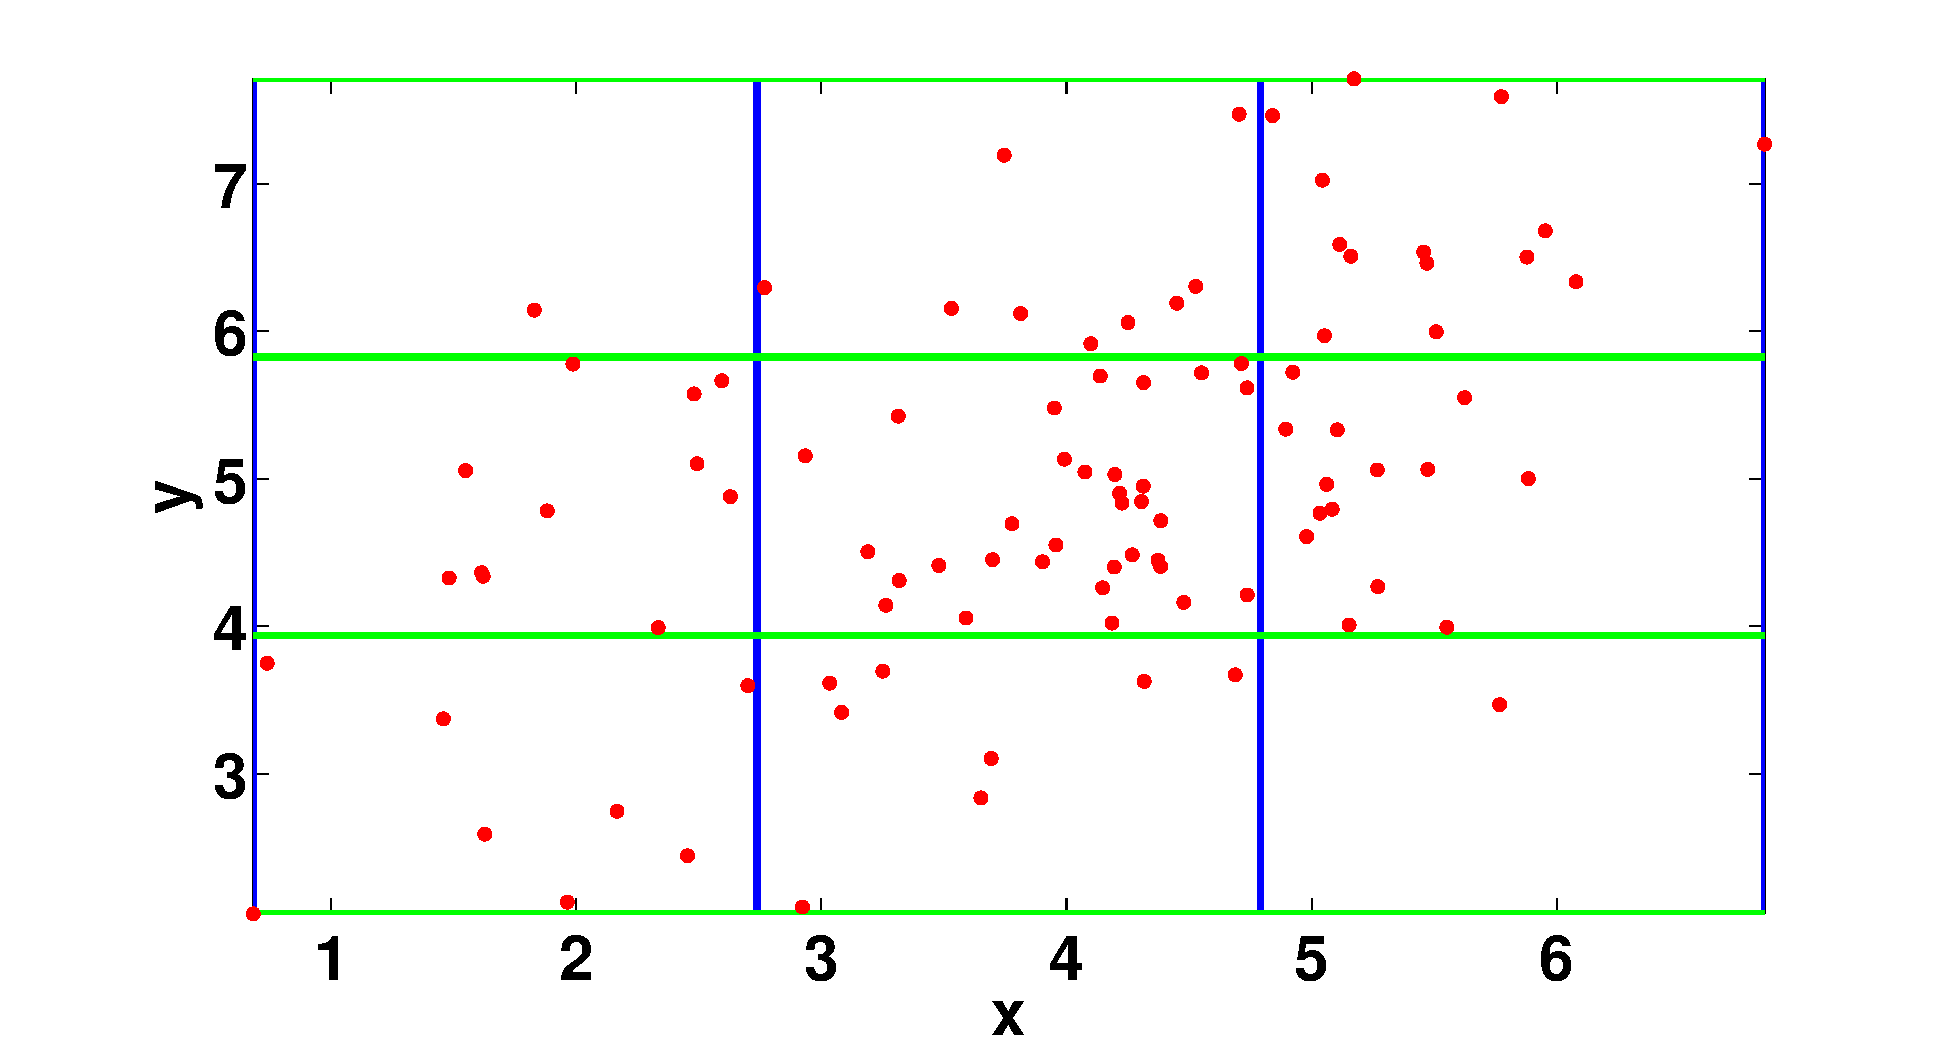
\includegraphics[width=0.55\textwidth]{equal-length.pdf}
   \label{fig: equal-length}
\end{figure}

\begin{figure}[!ht]
  \caption{Equal-depth}
  \centering
   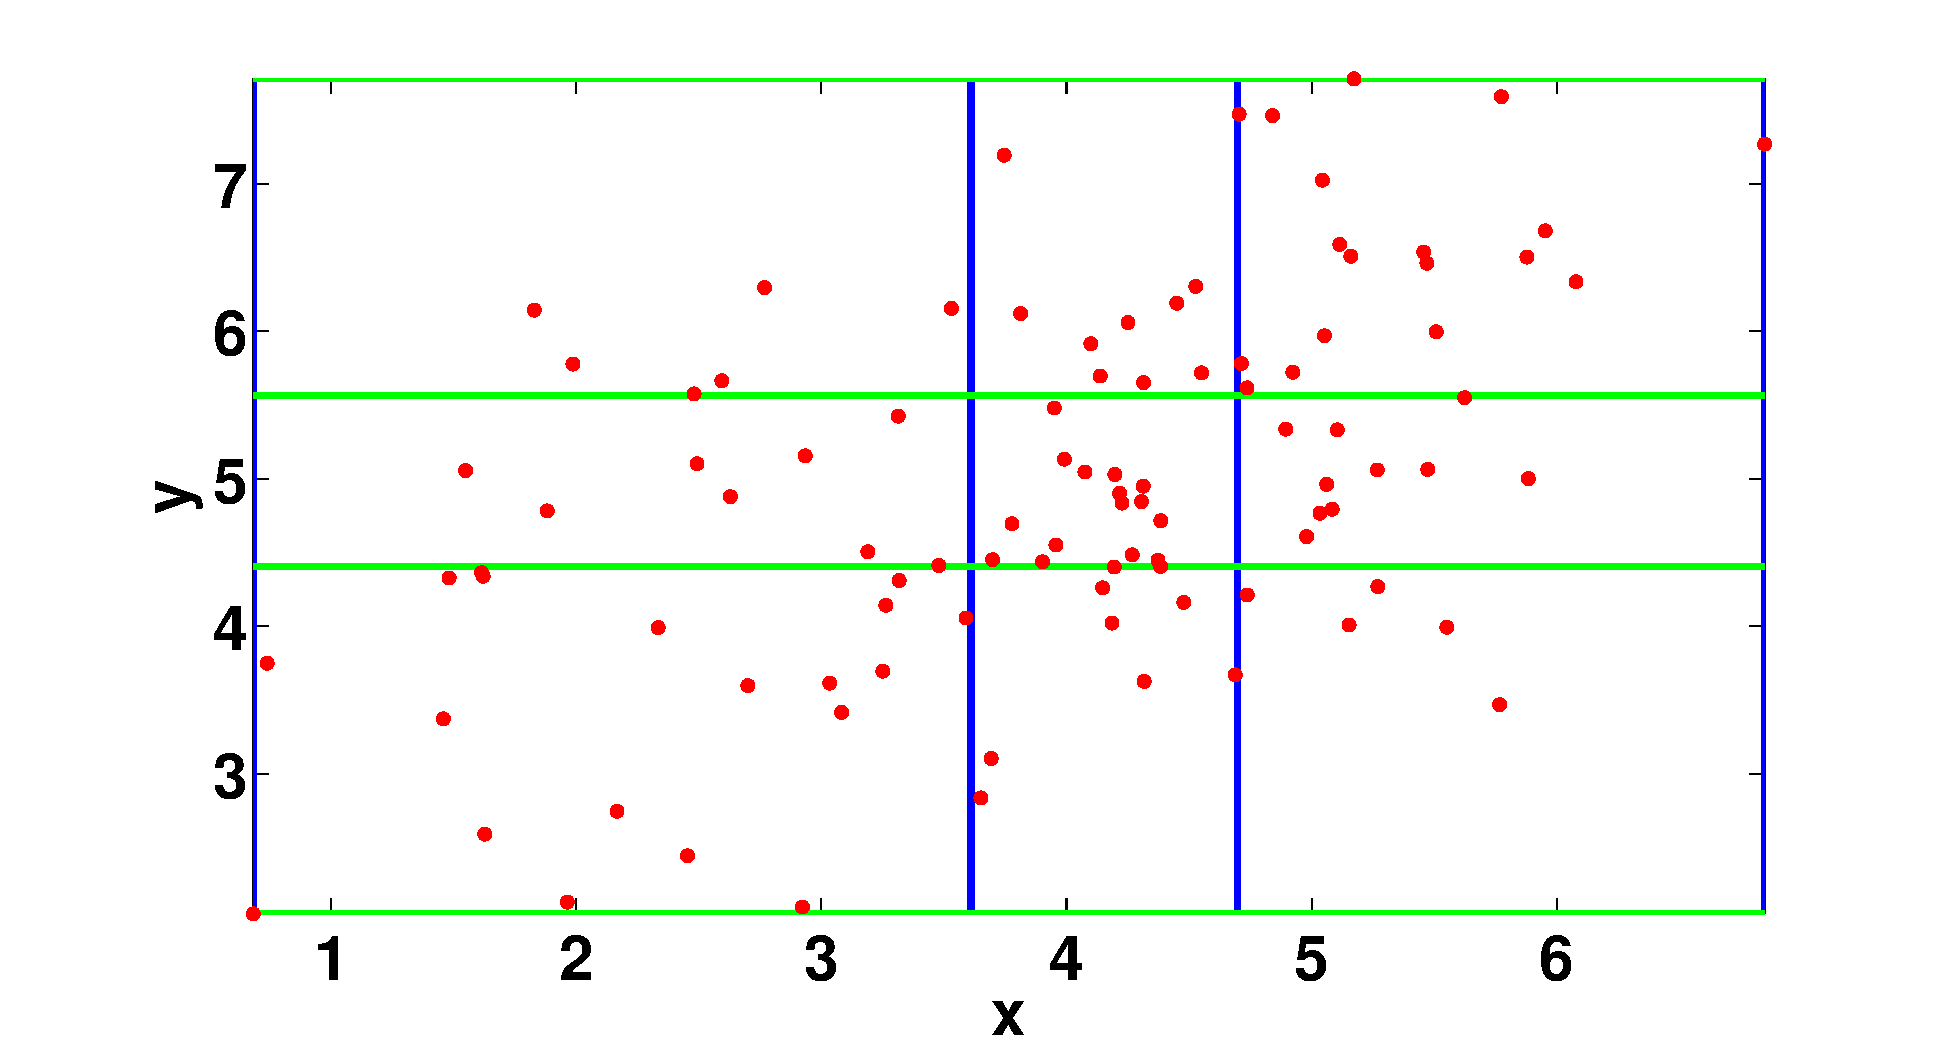
\includegraphics[width=0.55\textwidth]{equal-depth.pdf}
   \label{fig: equal-depth}
\end{figure}


\end{enumerate} 


\paragraph{ \text{2. }} Using weka.

\begin{enumerate}[(a)]
\item Data Preparation and integration \\

\textbf{Answer:} The steps I use for the data integration.
\begin{enumerate}[(i)]
\item Set merged file relation as \emph{hungarian-cleveland-heart-disease}
\item Check attributes. Note that attributes name "chest\_pain" and "cp" from these two files refer to same attributes. 
%\item Add one attributes to indicate the file source of each records, @attribute 'source' {hungarian, cleveland}.
\end{enumerate}

\item Description data summarization
\begin{enumerate}[(i)]
\item Study for example the age attributes. What is the mean? Its standard deviation? Its min and max? \\

\textbf{Answer:} Mean is 51.146 \\
 standard deviation is 9.08 \\
  min is 28, max is 77.
\item Provide the \textbf{five-number summary} of this attribute. Is this figure provide in Weka? \\

\textbf{Answer: } The five-number summary is: 
[min,first quartile, median,third quartile,max] =  [28, 44.0, 52.0, 58.0, 77]

The five-number summary is not provided in Weka.
\item Switch to the \textbf{Visualize} tab. What is the term used in the textbook to name the series of boxplots represented? By selecting the maximum jitter, and looking the \textbf{num} column, can you determine which attributes seem to be the most linked to heart disease? Paste the \textbf{boxplot} representing the attribute you find the most predictive of heart disease (Y) as a function of \textbf{num}(X). Does any pair of different attributes seem correlated? \\

\textbf{Answer:}
It has the name \textbf{scatter plot matrix}. \\
The attribute most linked to heart disease is \textbf{slope}. The boxplot is shown in Figure~\ref{fig: slope-correlated}. \\
Attribute \textbf{exang} and \textbf{slope} seem correlated as shown in Figure~\ref{fig: erlang-correlated}.


\begin{figure}[!ht]
  \caption{boxplot of num and slope attributes}
  \centering
   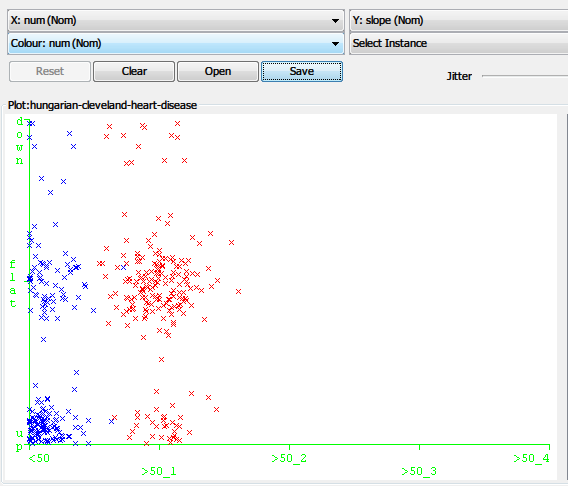
\includegraphics[width=0.7\textwidth]{slope-correlated.PNG}
   \label{fig: slope-correlated}
\end{figure}

\begin{figure}[!ht]
  \caption{boxplot of exang and slope attributes}
  \centering
   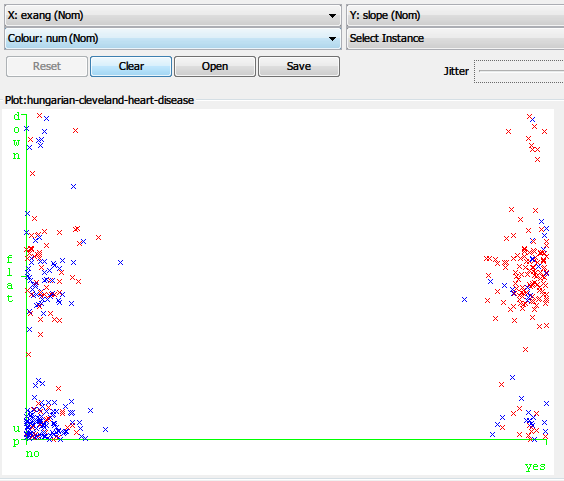
\includegraphics[width=0.7\textwidth]{erlang-vs-slope.PNG}
   \label{fig: erlang-correlated}
\end{figure}



\end{enumerate}

\item Data Preparation and cleaning
\begin{enumerate}[(i)]
\item Remove the missing values with the method of your choice, explaining which filter you are using and why you make this choice. Document what you did in your homework solution. \\

\textbf{Answer:} \\
I use filter \textbf{RemoveWithValues}, in the setting of this filter, \textbf{splitPoint} is used to filter numeric values, instances with values smaller than given value will be selected; \textbf{invertSelection} is used to invert the selection; \textbf{matchMissingValues} is sued to match instances with missing values. Note that it is independent of \textbf{invertSelection}, i.e., \textbf{invertSelection} will not affect the selection result of \textbf{matchMissingValues}.

I takes the following steps to filter the missing value instances:
\begin{itemize}
\item step 1: Choose \textbf{RemoveWithValues} filter, select the attributes which contains the most missing instances (attribute ca, index 12), set \textbf{matchMissingValues} as true, the final setting is, "RemoveWithValues -S 0.0 -C 12 -L first-last M". After this step, there are only 301 instances remaining.
\item Step 2: continue to select attributes to match missing values until there are no missing values in the instances. I select attribute \textbf{thal} next, note that since it is not numeric value, all its instances will be selected if the split point is set as 0.0, thus we need to set the  \textbf{invertSelection} as true to invert the selection. Finally, there are 297 instances remaining.
\end{itemize}

\item Past a screenshot of the first 10 rows of this clean dataset. \\

\textbf{Answer: } It is shown in Figure~\ref{fig: clean}.
\begin{figure}[!ht]
  \caption{First 10 rows of clean dataset}
  \centering
   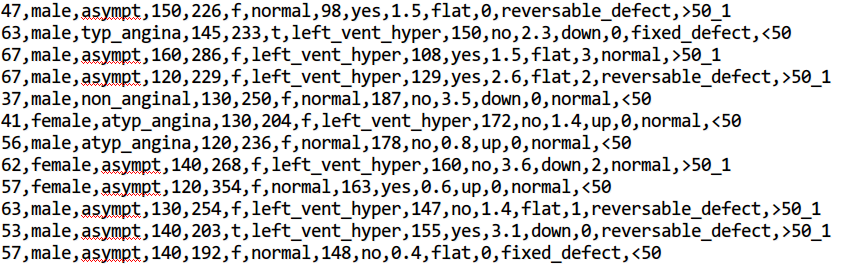
\includegraphics[width=0.98\textwidth]{filter-missing-values.PNG}
   \label{fig: clean}
\end{figure}

\end{enumerate}

\item Data preparation: transformation
\begin{enumerate}[(i)]
\item \textbf{Attribute construction} - for example adding an attribute representing the sum of two other ones. Which \textbf{Weka filter} permits to do this?\\

\textbf{Answer:} \textbf{AddExpression} filter.
\item Normalize an attribute. Which \textbf{Weka filter} permits to do this? Can this filter perform Min-max normalization? Z-score normalization? Decimal normalization? Provide detailed information about how to perform these in Weka. \\

\textbf{Answer: } \textbf{Normalize} filter can be used to normalize an attribute. It \textbf{can} perform min-max normalization and decimal normalization, but \textbf{cannot} perform Z-score normalization. 
\textbf{Standardize} filter can perform Z-score normalization. For decimal normalization, we select filter \textbf{Normalize}, and set the scale as 2, set the translation as -1, this will create the normalize range [-1,+1]. For the other normalization, we can apply the filters directly.
 
\item Normalize all real attributes in the data set using the method of your choice - State which one you choose. \\

\textbf{Answer: } I select the filter \textbf{Normalize}, and using the default setting with scale set as $1$ and translation set as $0$.
\item Save the normalized dataset into heart-normal.arff, and paste here a screenshot showing at least the first 10 rows of this dataset. \\

\textbf{Answer: } It is shown in Figure~\ref{fig: normal}.
\begin{figure}[!ht]
  \caption{First 10 rows of heart-normal.arff}
  \centering
   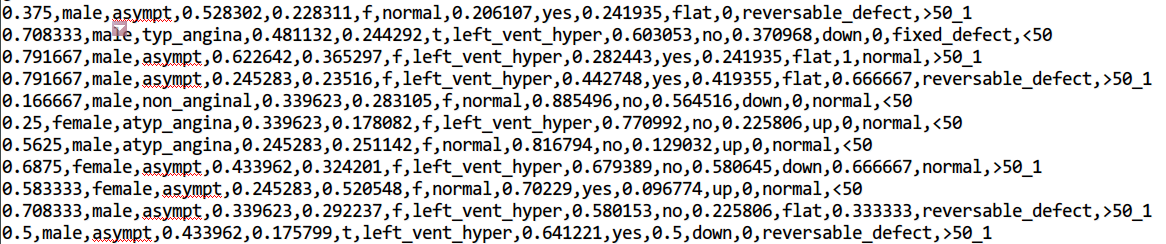
\includegraphics[width=0.98\textwidth]{normal-real.PNG}
   \label{fig: normal}
\end{figure}



\end{enumerate}

\item Data preparation: reduction \\
How to perform sampling with Weka filters? Can it perform the two main methods: \textbf{Simple Random Sample Without Replacement}, and \textbf{Simple Random Sample with Replacement}. Report your findings. \\

\textbf{Answer:} Filter \textbf{Resample} can perform sampling. It can perform both of these two main methods. The setting \textbf{noReplacement} is set true when perform sampling without replacement, and set false when perform with replacement. The attribute \textbf{sampleSizePercent} is used to set the size of sample. 

\end{enumerate}


\paragraph{\textbf{3. }} For the Clevelandheart data, use Weka to perform Principal Component Analysis 
\begin{enumerate}[(a)]
\item Keep only attribute(in the new space) that represent up to $70\%$ of the total variance \\

\textbf{Answer: } Apply "PrincipalComponent" filter, and set \emph{variance covered} field as 0.7
\item Remove the rest of the attributes and save the resulting data set.
\item Reconstruct the approximate original dataset. \\

\textbf{Answer: } We use \textbf{"Select attributes"} option, and use \textbf{PrincipleComponents} filter, and set standard deviation as $0.7$, and set \textbf{"transformBackToOrignal"} as true. The first 10 rows of reconstructed data are shown in Figure~\ref{fig: reconstruct}.

\begin{figure}[!ht]
  \caption{First 10 rows of reconstruct data set}
  \centering
   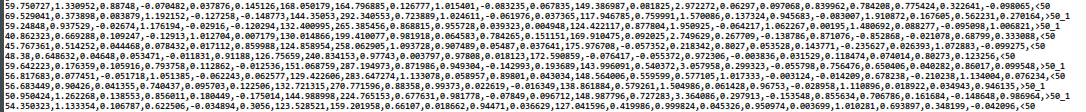
\includegraphics[width=1\textwidth, height = 1.1 in]{Reconstruct.PNG}
   \label{fig: reconstruct}
\end{figure}


\item Compute the distance (Enclidian) between every vector in the original Cleveland set and the approximate one. Report the average and standard deviation of the set of distances. Report the three records with highest distance between approximation and the original. \\

\textbf{Answer: } Let $X_1$ be the vector of the original data, and $X_2$ be the vector of the approximate one. Here $X_1$ is the reconstruct dataset that represent $100\%$ of the total variance. Then we compute the Euclidean distance between each corresponding row vector. We have:
\begin{itemize}
\item average distance: 35.7906245546
\item standard deviation:20.9852626932
\item the three records with highest distance: 175.71812427, 134.38525847,115.11248262.
\end{itemize}
\end{enumerate}
\end{document}

%%%%%%%%%%%%%%%%%%%%%%%%%%%%%%%%%%%%%%%%%%%%%%%%%%%%%%%%%%%%%%%%%%%%%%%%%%%%%%%% 